% \documentclass[letterpaper, twocolumn]{article}
\documentclass[sigconf]{acmart}


\usepackage{algorithm}
\usepackage{algpseudocode}
\usepackage{graphicx} 	% 1
\usepackage{wrapfig}
\usepackage{float} 		% to force figure placement
\usepackage{subcaption} % for the subfigure
\usepackage{amsmath} 	% to use \text{} command in math environment instead of \textrm{}
\usepackage{xcolor}
\usepackage{soul}       % for highlighting
\usepackage{xspace}
\usepackage{siunitx}
\usepackage[inline]{enumitem}
\usepackage{tikz}
%%%% Control the packages behavior
%\graphicspath{{../figures/}}

%\usepackage{booktabs} % For formal tables
%\usepackage{amsmath}
%\usepackage{hyperref}
%\usepackage{amssymb}
%\usepackage{tikz}
%\usepackage{pgfplots}
%\usepackage{lipsum}
%\usepackage{siunitx}
%\usepackage{subfig}
%\usepackage{flushend}
%\usepackage{libertine}
%\setlist{itemjoin ={,\enspace},itemjoin* = { and\enspace}}


%% New command for TODOs
\newcommand{\todo}[1]{}
\renewcommand{\todo}[1]{{\color{red} [{#1}]}}
\newcommand{\checkit}[1]{\textcolor{red}{Check---} \hl{#1}} 
\DeclareRobustCommand*\circled[1]{\tikz[baseline=(char.base)]{
            \node[shape=circle,draw,inner sep=1pt] (char) {#1};}}
\newcommand{\sys}{CIS\xspace}
\newcommand{\fullsys}{Coalesced Intermittent Sensor\xspace}
%\newcommand{\fullsys}{\sys: Battery-less Distributed Microphone}
%\newcommand{\fullsys}{Distributed Batteryless Intermittent Sensors}
%\newcommand{\fullsys}{Distributed Intermittent Systems: Theory and Practice}

\begin{document}

\title{Continuous Sensing on Intermittent Power} 

%\affiliation{\institution{Delft University of Technology}}
%\email{a.y.majid@tudelft.nl}
%
%\author{Patrick Schilder}
%\affiliation{\institution{Delft University of Technology}}
%\email{PATRIC@student.tudelft.nl}
%
%\author{Przemys{\l}aw Pawe{\l}czak}
%\affiliation{\institution{Delft University of Technology}}
%\email{p.pawelczak@tudelft.nl}
%
%\renewcommand{\shortauthors}{A.Y. Majid et al.}

%for single author (just remove % characters)
% \author{
% {\rm Amjad Yousef Majid}\\
% Delft University of Technology
% \and
% {\rm Patrick Schilder}\\
% Delft University of Technology
% % copy the following lines to add more authors
% \and
% {\rm Koen Langendoen}\\
% Delft University of Technology
% } 

\author{Amjad Yousef Majid}
\email{a.y.majid@tudelft.nl}
% \orcid{1234-5678-9012}
\affiliation{%
  \institution{Delft University of Technology}
}
\author{Patrick Schilder}
\email{p.t.schilder@student.tudelft.nl}
\affiliation{%
  \institution{Delft University of Technology}
}
\author{Koen Langendoen}
\email{k.g.langendoen@tudelft.nl}
% \orcid{1234-5678-9012}
\affiliation{%
  \institution{Delft University of Technology}
}
\author{Stephan Wong}
\email{j.s.s.m.wong@tudelft.nl}
% \orcid{1234-5678-9012}
\affiliation{%
  \institution{Delft University of Technology}
}


%\keywords{}

\begin{abstract}
The main obstacles to achieve truly ubiquitous sensing are (i) the limitations of battery technology - batteries are short-lived, hazardous, bulky, and costly - and (ii) the unpredictability of ambient power. The latter causes sensors to operate intermittently, violating the availability requirements of many real-world applications. 
%
In this paper, we present the \textit{\fullcis} (\cis), an
intermittently-powered ``sensor'' that senses continuously! Although
a single node will frequently be off charging, a group of nodes can
--in principle-- sense 24/7 provided that their awake times are spread
apart. As communication is too expensive, we rely on inherent component
variations that induce small differences in power cycles. This basic
assumption has been verified through measurements of different nodes
and power sources. However, desynchronizing nodes is not enough.
%
An important finding is that a \cis designed for certain (minimal)
energy conditions will become synchronized when the available energy
exceeds the design point. Nodes employing a sleep mode (to extend
their availability) do wake up collectively at some event, process it,
and return to charging as the remaining energy is typically too low to
handle another event. This results in multiple responses (bad)
and missing subsequent events (worse) due to the synchronized charging.
To counter this undesired behavior we designed an algorithm to estimate the number of active neighbors and respond proportionally to an event. 
We show that when intermittent nodes randomize their responses to events, in favorable energy conditions, the \cis reduces the duplicated captured events by 50\% and increases the percentage of capturing entire bursts above 85\%. 


% The main obstacles to achieve truly ubiquitous sensing are (i) the limitations of battery technology - batteries are short-lived, hazardous, bulky, and costly - and (ii) the unpredictability of ambient power. The latter causes sensors to operate intermittently, violating the availability requirements of many real-world applications. 
% 
% In this paper, we present the \textit{\fullcis} (\cis), an intermittently powered ``sensor'' that senses continuously!
% Our key observation being that, the power cycles of energy-harvesting battery-less devices do not show correlation even when they are drawing energy from the same source, running the same application, and in close proximity.
% We challenged our observation using different real hardware and energy sources and showed that this observation holds.
% 
% Another important finding is that a \cis designed for certain (minimal) energy conditions requires no explicit spreading of awake times due to embedded randomness in the powering subsystem. However, when the available energy exceeds the design point, nodes employing a sleep mode (to extend their availability) do wake up collectively at the next event. This synchronization leads to problems as multiple responses will be generated, and -worse- subsequent events will be missed as nodes will now recharge at the same time.
% To counter this unwanted behavior we designed an algorithm to estimate the number of active neighbors and respond proportionally to an event. 
% We show that when intermittent nodes randomize their responses to events, in favorable energy conditions, the \cis reduces the duplicated captured events by 50\% and increases the percentage of capturing entire bursts above 85\%. 

\end{abstract}
%
% The code below is generated by the tool at http://dl.acm.org/ccs.cfm.
% Please copy and paste the code instead of the example below.
%
\begin{CCSXML}
<ccs2012>
 <concept>
  <concept_id>10010520.10010553.10010562</concept_id>
  <concept_desc>Computer systems organization~Embedded systems</concept_desc>
  <concept_significance>500</concept_significance>
 </concept>
 <concept>
  <concept_id>10010520.10010575.10010755</concept_id>
  <concept_desc>Computer systems organization~Redundancy</concept_desc>
  <concept_significance>300</concept_significance>
 </concept>
 <concept>
  <concept_id>10010520.10010553.10010554</concept_id>
  <concept_desc>Computer systems organization~Robotics</concept_desc>
  <concept_significance>100</concept_significance>
 </concept>
 <concept>
  <concept_id>10003033.10003083.10003095</concept_id>
  <concept_desc>Networks~Network reliability</concept_desc>
  <concept_significance>100</concept_significance>
 </concept>
</ccs2012>
\end{CCSXML}

\ccsdesc[500]{Computer systems organization~Embedded systems}
\ccsdesc[300]{Computer systems organization~Redundancy}
\ccsdesc{Computer systems organization~Robotics}
\ccsdesc[100]{Networks~Network reliability}

\keywords{ Embedded systems, Distributed intermittent computing}

\maketitle


\section{Introduction}
\label{sec:introduction}
Batteries may compromise the viability of sensor nodes in various ways. Batteries are bulky, short-lived, hazardous, and expensive. To ameliorate the battery problem, researchers have been investigating different alternatives to extend lifetime and reduce costs and form factor.  
The reduction in power consumption of recent microcontrollers (MCUs) and the advances in energy-harvesting (EH) circuitry have enabled the emergence of battery-free EH sensors. 
These sensors elide the constraints of batteries and extract power from ambient energy sources such as sunlight and RF emissions. 

Ambient energy sources provide perpetual power. However, ambient power is usually too weak to directly power a sensor node~\cite{liu2013ambient}.  Therefore, an EH  node first buffers the harvested energy until a usable amount has been accumulated; then it operates, for a short period of time, until the buffered energy has been exhausted~\cite{lucia2017intermittent}.  Consequently, battery-less EH sensors operate intermittently (Figure~\ref{fig:intermittent_opertaion}).

Intermittent power introduces a set of new challenges that are under ongoing investigation.
For example, \cite{lucia2017intermittent,ransford2011mementos,dino,colin2016chain,balsamo2014hibernus,rodriguez2018restop} studied the intermittent computation problem, which is concerned with the preservation of application progress and data consistency under frequent power failures; the authors of \cite{hester2017timely} investigated the timely operation challenge, which is concerned with data freshness after a power interrupt; 
and \cite{yildirim2018ink} introduced event-driven execution for the intermittent domain, which deals with input and output operations under arbitrarily-timed power loss.

Despite these notable advances, intermittently-powered sensors suffer from a new fundamental shortcoming: \textit{the intermittent availability of the system}. Being frequently off charging compromises the value of these devices. For example, a sensor that has a low probability (e.g., 10\%~\cite{coala}) to be available (on) when an event of interest occurs has no value. 
Overcoming the intermittent availability challenge without changing the size of the device or re-including batteries requires a novel approach that explores new design dimensions. 
%
\begin{figure}[b]
	\centering
		\includegraphics[width=\columnwidth]{figures/intermittent_operation}
		\caption{Harvested-energy profile. Ambient power is weak; therefore, it is usually buffered. The buffered energy is then consumed to operate the device. The operation period is often short as power consumption is much higher than the energy harvesting rate.}
		\label{fig:intermittent_opertaion}
\end{figure} 
%
\subsection{Vision and Application}
%
\begin{figure}[t]
	\centering
	\includegraphics[width=\columnwidth]{figures/smart_fabric}
	\caption{A \fullcis (\cis) is a group of intermittently-powered nodes that sense continuously despite the intermittent power supply. \cis exploits the inherent randomization of energy harvesting systems, if available, and introduces artificial randomization, when needed, to preserve continuous sensing.}
	\label{fig:smart_fabric}
\end{figure}
%
Miniaturized sensors are non-intrusive devices. Therefore,
they can be embedded in locations that are not suited for the others (enabling
new applications). Miniaturizing sensors, however, introduces the significant
challenge of powering them.
%
On the one hand, batteries make these sensors \emph{continuously}
available -for sensing opportunities-, but with an environmental footprint
and only for a short period of time.
% (even rechargeable batteries wear out after a few hundreds of charging cycles~\cite{aditya2008comparison}).
%(although new battery technology promise longer lifetime~\cite{jackson2018reconsidering, jackson_ipsn_2019}, new batteries are still (potentially hazardous) batteries, and battery waste is a rapidly growing problem). 
%
On the other hand, removing batteries and relying on ambient energy make them
available for a long period of time, but intermittently. 
%
Our vision\footnote{An alternative approach is to combine EH with a
(small) rechargeable battery~\cite{jackson2018reconsidering, jackson_ipsn_2019}.} is that by combining {\em multiple} battery-less EH sensors we can create a new {\em virtual} sensor that operates permanently (no batteries) and reliably (continuously available): we call this sensor the \emph{\fullcis} (\cis).

Sensors with such characteristics would allow us to add a cheap and maintenance-free sensing layer to many objects, making them smart and interactive. For example, one can imagine developing smart wallpaper that users can interact with. 
Smart wallpaper with embedded microphones can enable direct in-building human-to-object communication (Figure~\ref{fig:smart_fabric}). Such a permanently operating sensor can be deployed, for example, in kids' playgrounds to monitor their occupancy. These battery-less sensors can enable
interactive and safe-to-dispose sports rugs (that count how many times a person has jumped on them) or play rugs for kids.
In short, we would like to develop small sensors with permanent and continuous sensing capabilities.  
%
\subsection{Research Challenges}
Many sensing applications require the sensor to be available when there is a change in the monitored environment.
EH battery-less sensors can provide cheap and maintenance-free sensing, but they do not meet the availability requirements of many real-world applications. 

\noindent\textbf{C1-Approach continuous availability on intermittent power}: 
An EH battery-less sensor is frequently off, spending most of the time charging. One way to increase the availability of the system is by using multiple nodes.
However, coordinating the nodes' awake times using communication may introduce prohibitive overhead as a scattering algorithm must be regularly executed, and messages for synchronizing nodes' clocks and reserving time slots need to be repeatedly exchanged.
Thus, the challenge is \emph{can we exploit some of the inherent characteristics of EH battery-less sensors to distribute nodes' awake times without the need for communication?}

\noindent\textbf{C2-Continuous sensing on intermittently powered sensors:}  
Even when the collective availability of intermittent sensors approaches 100\%, the emerging overall sensing behavior may still be intermittent. 
Event-trigger sensors sleep in low-power mode waiting for an event to wake them up. 
When ambient energy rises, the EH rates of these sensors may equal (or approximate) their sleeping mode power consumption.
Under such energy conditions, these sensors become available for an extended period of time. 
Therefore, when an external event arrives, nodes respond collectively, which exhausts their energy buffers, making them unavailable for the next set of events. 
This is, particularly, a significant problem when events arrive in bursts, like a command of a few words (e.g., ``light on''). 
Thus, the challenge is, \emph{how to prevent EH battery-less sensors from synchronizing their power cycles on some of the incoming events?}

\noindent\textbf{C3-Efficient sensing on intermittent sensors:} 
One of the main factors that determine the intermittency pattern of an EH battery-less sensor is the richness of ambient energy. 
For example, at mid-noon under direct sunlight, even a small solar panel can power a sensor node continuously. 
In such conditions (favorable energy conditions), using plenty of intermittent sensors would only result in duplicated work that leads to duplicated messages when the data is being communicated to a sink node: a continuously-powered node acts as a gateway for such sensors to communicate with other layers of the Internet of Things. These messages will collide as they will be generated at approximately the same time, and if some of them are received by the sink, then they waste energy as they carry the same information. Thus, the challenge is, \emph{how to reduce the number of duplicated event detections?} 
%
\subsection{Contributions}
In this paper, we tackle the paradox of continuous sensing on intermittently-powered sensors. 
We studied the inter-relationship between the power cycles of EH battery-less devices, the emerging collective behavior, and the effect of the change in ambient energy on this behavior. In particular, this paper makes the following key contributions:
\begin{itemize}[leftmargin=*]
%
\item We show how to approach continuous sensing using multiple intermittently-powered sensors. 
For that, we \textbf{modeled} the collective effective availability---the system availability that leads to successful sensing---of a group of intermittent sensors and \textbf{validated} our models using simulation and on real hardware against different ambient energy sources. 
%
\item We introduce a new type of virtual sensor, showing its capabilities and limitations. This \textbf{\fullcis (\cis)} is the abstraction of a group of intermittently-powered sensors that achieves maximum statistical availability by exploiting (inherent) randomization to spread nodes' awake times uniformly.
% 
\item Contrary to common sense, we show how favorable energy conditions can deteriorate the performance of a \cis. We, therefore, equipped the \cis with \textbf{an new algorithm} that makes it ambient-energy aware. This algorithm enables the nodes to determine their own duty cycles (without requiring additional hardware), and the average number of alive nodes (without requiring communication). This information can effectively be used by the nodes to decide when to back off to avoid duplicated event detection and availability interruptions (implicit synchronization in favorable harvesting conditions).
%
\item We prototype, evaluate, and demonstrate the feasibility of the \fullcis concept in the form of a voice-control commands recognizer, the \textbf{\fullCIM} (\textbf{\cim}). 
We chose to develop a command recognizer as 
voice is a natural way for the human to interact with small devices. Moreover, words allow us to easily experiment with individual event arrivals and events that arrive in bursts. 
However, the goal of this paper is \emph{not} to present a novel word recognition technique. 
Instead, we adapt a classical word recognition algorithm to make it power-failure immune. Yet, our \cim prototype is the first intermittent command recognizer, shedding light on the potential of intermittent systems. 

\end{itemize}























%\section{Batteryless Distributed Sensing}
%\label{sec:disSensing}
%\subsection{Events Classification}

Given an intermittent device with a certain on-time duration ($d_{on}$), we can classify external events from the device perspective as follows:
\begin{itemize}
		\item \textit{Short events}---The event duration is shorter than the on-time of an intermittent device ($d_{on} < t_{on}$). This event can be (i) repetitive, i.e. the acoustic wave caused by a deformed gear tooth; or (ii) non-repetitive, i.e. single word command for a voice assistant.  

		\item \textit{Long events}---The event duration is much longer than the on-time of an intermittent device ($d_{on} > t_{on} $). These events can be (i) simple, such that capturing a small fraction of the event is sufficient to get all the information, i.e. vibration; or (ii) complex, such that capturing the entire event is required for correct interpretation, i.e. a command of several words to a voice assistant system. 
\end{itemize}

\subsection{Intermittent devices classifications}
Intermittent devices can be classified based on the relation between their on/off cycles and the occurrence of external events:  
\begin{itemize}
		\item An \textit{Event oblivious} intermittent device starts running once its energy buffer is full, regardless of the occurrence of an external event. In other words, the dispersion of the on-times of this type of intermittent devices is unaffected by the occurrence of external events. 
		\item An \textit{Event aware} intermittent device enters sleep mode once its buffer is full and upon the occurrence of an external event starts software execution. The power cycles of this type of intermittent devices tend to synchronize as their up times is triggered by an event.  

\end{itemize}

Events aware intermittent devices tend to have a longer effective on-time: the time needed to capture an event and save the data in memory.
%
%

%A fundamental limitation of intermittent devices are their inherent repeated absence. A natural way to combat this limitation is by grouping these tiny devices together and abstracting them as a single \emph{intermittent distributed system}. The collective on-time of these devices should approach continuous time as their number increases. However, the on-time and off-time of  distributed intermittent systems depend on the environment and the load. As such, we do not expect, for example, a linear relationship between the number of nodes and the overall on-time. 

%An intermittent device uses a capacitor (a buffer) to store energy and, usually, the capacitor has operational and shutdown thresholds (Figure\,\ref{fig:powerCycle}). 
The on-time evolution of a event-oblivious distributed intermittent system, as more nodes join, depends on the special diversity of its individual nodes.
%Depending on their spatial diversity, the nodes of a distributed intermittent system can experience the same energy harvesting conditions or not.
\subsection{Spatially Diverse Intermittent Devices}
%
\begin{figure}
	\centering
		\includegraphics[width=\columnwidth]{figures/coverage.pdf}
	\caption{The on-time of a distributed intermittent system.}
	\label{fig:independentCoverage}
\end{figure}
%
\checkit{If the nodes are spatially diverse such that their energy harvesting rates are statistically different, then we can assume that the power cycles of the nodes are independent and uniformly distributed over the overall distributed system's power cycle}---When all the nodes power up and shutdown again\footnote{\todo{maybe it is better to define it as the mean of the individual power cycles}}. 
When the power cycles are uniformly distributed, adding a node increases the average on-time as follows, 
%
\begin{equation}
\delta t = \frac{t_{off}}{s_{pc}} * n_{on}
		\label{eq:indCov}
\end{equation}
%
where $t_{off}$ is the off-time of the distributed system, $s_{pc}$ is the period of the distributed system's power cycle, $n_{on}$ is a node on-time, and $\delta t$ is the time gain of the distributed intermittent system.

As Figure\,\ref{fig:independentCoverage} shows adding nodes to intermittent distributed systems increases its overall on-time, and consequently, its responsiveness. It is also clear that the benefit of an additional node is inversely proportional to the distributed system's on-time. Equation~\ref{eq:indCov}, however, holds only when nodes wake-ups approximate a uniform distribution. \checkit{When the nodes are in close proximity, we cannot model their power cycles as a random variable drawn from a uniform distribution because their energy charging rates are correlated}. 

\subsection{Spatially Invariant Intermittent Devices}
%
\begin{figure}
	\centering
	\begin{subfigure}[t]{0.49\columnwidth}
		\includegraphics[width=\textwidth]{figures/offtime.pdf}
			\caption{off-time length distribution}
		\label{fig:offtime}
	\end{subfigure}
	\begin{subfigure}[t]{0.49\columnwidth}
		\includegraphics[width=\textwidth]{figures/ontime.pdf}
		\caption{on-time length distribution}
		\label{fig:ontime}
	\end{subfigure}
		\caption{The distributions of the operational stages of a distributed intermittent system.}		
\end{figure}
%
To understand how the on-time of a distributed intermittent system evolves when devices' power-ups are correlated, we need to investigate the \checkit{variance} of the off-time and on-time intervals.  

The \textit{off-time} of an intermittent device depends only on the environment: high charging rate results in short charging time and vice versa. Hence, we may model the off-time as a random variable drawn from a normal distribution (Figure\,\ref{fig:offtime}). The \textit{on-time}, however, depends on the buffered energy---the harvested energy while the device is off---; the harvested energy while the device is on, which only prolongs the execution; and the load of the device. Therefore, if we assume the load is constant, then we can model the on-time as a random variable drawn from a gamma distribution can be more appropriate (Figure\,\ref{fig:ontime}). Another important factor is \textit{the relation} between the off-time and the on-time. Short off-time indicates a high charging rate. A high harvesting rate results in a non-negligible amount of the harvested-while-executing energy. This energy lengthens the on-time. Therefore, we can conclude that there is an inverse relationship between the on-time and the off-time. \checkit{By considering these three factors (on-time, off-time, and their relation), we can model the variation in intermittent devices' power cycles as a normal distribution}. As a result, when charging rates are correlated, the power-ups of intermittent nodes will tend to cluster around the mean instead of spreading over the entire power cycle of the distributed intermittent system. 

\todo{relocate the following paragraph}
To flatten the normal distribution we need to add another random variable that is drawn from a uniform-like distribution. To achieve that, we further randomize the length of the on-time of intermittent nodes by injecting delays---putting the nodes into sleep mode---upon devices' power-ups (Figure\,\ref{fig:spreading}). The maximum delay that can be added is bounded by the buffer size and the minimum energy consumption of the load. The length of this delay represents the spreading factor by which we spread the original distribution of the nodes' wake-ups.  


\todo{Update equation 1 to include the spreading factor}

\begin{figure}
	\centering
		\includegraphics[width=\columnwidth]{figures/spreading.pdf}
	\caption{Spreading normally distributed intermittent devices over a larger range by injecting delays with a uniformly distributed lengths.}
	\label{fig:spreading}
\end{figure}
%The energy charging rate is environment dependent, while the discharge rate is load dependent. If we assume ambient energy does not fluctuate very quickly, then we can conclude that there is an inverse relationship between the on-time (discharging time) and the off-time (charging time). Short charging time means fast energy shots arrival. High energy harvesting rate prolongs discharge (execution) time, as the device harvests a nonible amount of energy while executing. 





















\section{Coalesced Intermittent Sensing}
\label{sec:coalInterSen}
\begin{figure}[t]
	\centering
		\begin{subfigure}{\columnwidth}
			\includegraphics[width=\columnwidth]{figures/PowerCycleIntermittentSystem}
			\caption{When \sys does polling-based sensing, its energy consumption profile has, generally, two distinct rates: zero when it is charging, and a maximum when it is sensing.}
			\label{fig:pollingBasedSensing}
	\end{subfigure}
	\begin{subfigure}{\columnwidth}
		\includegraphics[width=\columnwidth]{figures/PowerCycleIntermittentSensor}
		\caption{When \sys does event-based sensing, it stays in low-power mode waiting for an external event to wake up the node. Consequently,  it has three distinct energy consumption rates: zero when it is charging, a maximum when it is sensing, and an in-between when it is sleeping. In favorable energy conditions, the sleeping mode may cause intermittent nodes to synchronize their power cycles on external events and miss the next ones.}
		\label{fig:eventBasedSensing}
\end{subfigure}
		\caption{\fullsys (\sys) energy profile for different sensing strategies. Green bars highlight successful sensing operations  while the red bar shows a failed sensing attempt due to insufficient buffered energy.}
		\label{fig:cisPwrCycle}
\end{figure} 
%
The \fullsys (\sys) is the abstraction of a group of battery-less intermittent sensor nodes seeking to provide continuous availability to the user. The key to success is to exploit the properties (i.e.\ randomness) of the ambient energy source to arrive at a uniform spreading of the awake times of the individual senor nodes to achieve the maximum coalesced availability. To this end we will first analyze the energy-consumption life cycle of an intermittently-power node, as well as the joined availability of multiple nodes. Then we will point out a practical aspect that is often overlooked; when intermittent nodes operate in favorable ambient conditions, their uncorrelated behavior changes due to the extra energy leading to synchronized patterns that need to be scrambled by introducing artificial, controlled randomization.


%\sys seeks to offer continuous sensing despite relying on ambient energy: an unpredictable and marginal power source. 
%orchestrates its nodes power cycles using a distributed approach (instead of relying on a master powerful node to coordinate coalesced nodes activities). 
%\sys seeks maximum time span of its underlying coalesced nodes through a distributed approach instead of a master node that orchestrates coalesced nodes on/off cycles. 
%\textcolor{red}{\bf Stephan: maybe add a sentence to introduce the upcoming (sub)sections.}

\subsection{Energy consumption}
%
\todo{reevaluate the importance of this paragraph and its location accordingly}
An intermittent sensor has a limited energy budget per power cycle. When it is tasked with a polling-based sensing activity, its energy consumption, generally, switches between two levels: zero when charging and maximum when it activates its microcontroller for data acquisition and processing, see Figure~\ref{fig:pollingBasedSensing}. (Note that we assume that the microcontroller is the dominant energy consumer module of a node.) However, in event-based sensing, a node puts its microcontroller into low-power mode and waits (or listens) for an external event to wake up the microcontroller. In case of the command recognizer we exploit the microphone's wake-on-sound feature to send an interrupt to the microcontroller, which will then start recording the sound samples from the microphone. This hardware approach is most energy efficient, but can be mimicked in software by periodic polling (i.e.\ acquiring 1 sound sample and checking if it exceeds the acoustic noise floor). This wake-on-event style of operation is important as the minimal energy consumption during sleep significantly prolongs the period during which an event can be handled, see Figure~\ref{fig:eventBasedSensing}. Although in reality the sleep and active phases draw quite different levels of power (128 vs. 849~$\mu$W on our hardware, see Table~\ref{tab:power_usage}) we will model the life cycle of a sensor node simply as an on-period followed by an off-period (in which the node recharges its energy buffer) as that suffices to analyze the collective availability of a \sys.
%The idle listening mode, which is important for successful sensing, complicates the design of the \sys.

\subsection{Coalesced availability}
\label{subSec:availability}
%
\begin{figure}[t]
		\centering
		\includegraphics[width=\columnwidth]{figures/cisOntime}
		\caption{A \fullsys's availability is the emerging collective on-time of its intermittent nodes' on-times. The difference between the power cycles leads to a constant relative shift between the nodes duty cycles. This, in turn, causes their on-times to be uniformly distributed on the overall power cycle. The red bars indicate a minimum \sys time span---\sys's nodes are overlapping---whereas the green bars show the maximum time span of the \sys.}
		\label{fig:cisOntime}
\end{figure} 
%
\todo{Additional parameter: minimum time is needed to successfully capture an event. Nodes are uniformly distributed, and thus its overlapping intervals are also uniformly distributed. As such, for successful capturing, the overlapping interval must exceed the minimum time required for capturing an event. Another approach is to monitor the voltage level on the cost of additional hardware, complexity }

The \sys's on-time is the projection of its underlying intermittent nodes' on-times on the time axis. The \sys's on-time ranges from minimum (when all nodes on-times cluster together, see the red regions in Figure~\ref{fig:cisOntime}) to the maximum (when the overlapping between its nodes on-times is zero or when continuous availability is reached, highlighted with a green color in Figure~\ref{fig:cisOntime}). Two broad strategies for minimizing overlapping, hence, maximizing \sys availability, can be imagined: 
\begin{enumerate}[label=\roman*.]%[wide, labelwidth=!, labelindent=0pt]
%
		\item \textit{Explicit on-time division strategy}: Recent advancements in timing intermittent operations enable intermittent nodes to measure their on and off times with the help of an external ultra-low-power timer~\cite{hester2017timely}. Similar breakthroughs in passive communication enable ultra-low-power message exchange between battery-less nodes~\cite{li2015retro}. Intermittent nodes can use these advancements to apply a time-division multiplexing strategy to explicitly avoid overlapping on-times. For example, a node calculates its average on-time $\overline{t_{on}}$ and off-time $\overline{t_{\it off}}$ for $N$ power cycles. Then it measures the time difference between its power-up and the intended transmitting time $\Delta\,t$. Subsequently, it encodes the information $({\overline{t_{\it off}}, \overline{t_{on}}, \Delta\,t})$ in a message and broadcasts it. When a node receives this message it will have full knowledge about the transmitting node's power cycle. It can then alter its power cycle, relative to the transmitting nodes cycle, by either increasing (or decreasing) its power consumption to shorten (or lengthen) its on-time or shift its power cycle to a different time slot. This approach, obviously, assumes relatively stable nodes' power cycles. Assuming $N$ nodes observe the same on -and off- periods, the coalesced availability (their collective on-time) would be $N$ times the duty cycle of a node (or 100\% if the total length of the on-times exceeds a single power cycle).
%
\begin{figure}
		\centering
		\includegraphics[width=\columnwidth]{figures/cisModel}
		\caption{\fullsys availability percentage for a different number of nodes and different duty cycles. The nodes are uniformly distributed and the \sys on-time evolves, when adding new nodes, according to the equation~\ref{eq:cisModel}.}
		\label{fig:cisModel}
\end{figure} 
%
		\item \textit{Implicit on-time division strategy}: With no information being exchanged between intermittent nodes, the best \sys can do is to uniformly distribute its node's on-times and maintaining this distribution over time. The key observation to uniformly distribute the nodes' on-times is to ensure that their power cycles are different. This can be achieved by forcing intermittent nodes to go into low-power mode upon power-ups. The length of this mode is randomly chosen for each node. This will change the length of the nodes on-times and, consequently, alter their power cycles. Figure~\ref{fig:cisOntime} shows the scenario of two intermittent nodes with different power cycles. Node 1 has a power cycle of 6 units of time and an on/off cycle of $\frac{1}{3}$. Node 2 has a power cycle of 5 units of time and an on/off cycle of $\frac{1}{5}$. Following the time axis from the left, we can see that the position of the on-time of Node 2 is shifted by 1 unit of time after each power cycle of Node 2. This implies that the on-times of the two nodes are $\frac{1}{3}$ of the time cluster together and $\frac{2}{3}$ of the time they are apart. If we extend the previous scenario to three or more nodes then the on-time of the resulting \sys can be described with the following formula,
				
\begin{equation}
	t_\text{on}(N) = t_\text{on}(N-1) + \frac{t_\text{off}(N-1)}{t_\text{off}(N-1)+t_\text{on}(N-1)} \times t_\text{on}(1),
		\label{eq:cisModel}
\end{equation}
where $N \in \mathbb{N}$ and  $t_\text{on}(N)$ is the on-time of a \sys with $N$ intermittent nodes. For the initial case where $N=1$ we define $t_\text{on}(0)\coloneqq 0$ and $t_\text{off}(0) \coloneqq 1$.
				
In addition to characterizing the availability of a \sys, equation~\ref{eq:cisModel} also states that the benefit of adding a node to the \sys is proportional to the \sys's off-time. In Figure~\ref{fig:cisModel} \sys availability percentage for different duty cycles and different number of intermittent nodes are shown.
\end{enumerate}
%s
\todo{this paragraph disconnect the paragraph below it from the one above it} There is a clear trade-off between the aforementioned methods. While the explicit control method provides fine control over the system 
distribution and therefore requires less number of nodes than the implicit control method, the implicit control method does not depend on the ability to communicate between the nodes and therefore it is simpler and more energy efficient. Since inter-node communication is beyond the capabilities of most of today's intermittent nodes, we focus on the implicit approach.
 
%Although the implicit method is relatively simple to implement and explore, the explicit control method is not a far-fetched idea considering the recent advancements in passive communication and intermittent timing. However, we opt to explore the implicit distribution control method as the hardware used to demonstrate the feasibility of passive light communication and ambient RF backscattering are not open source and re-making it is beyond the scope of this study.

\begin{figure}[t]
		\begin{subfigure}{\columnwidth}
			\centering
			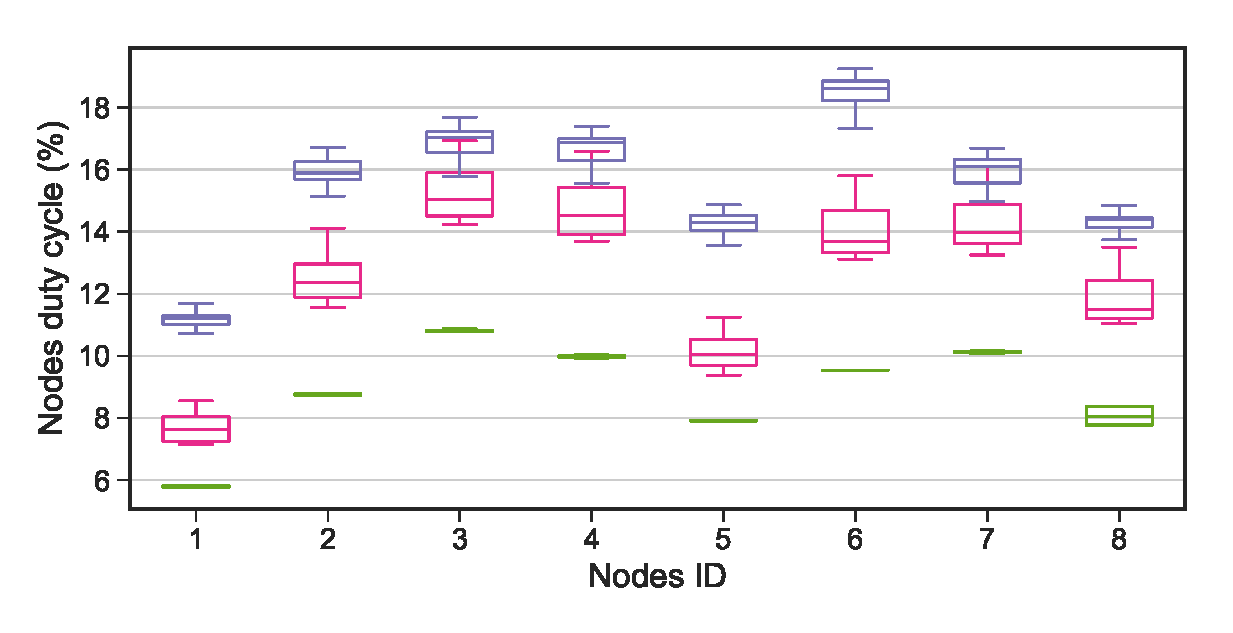
\includegraphics[width=\textwidth]{figures/natural_light_nodes_duty_cycles}
				\caption{light}
		\end{subfigure}\hfill
		\begin{subfigure}{\columnwidth}
			\centering
			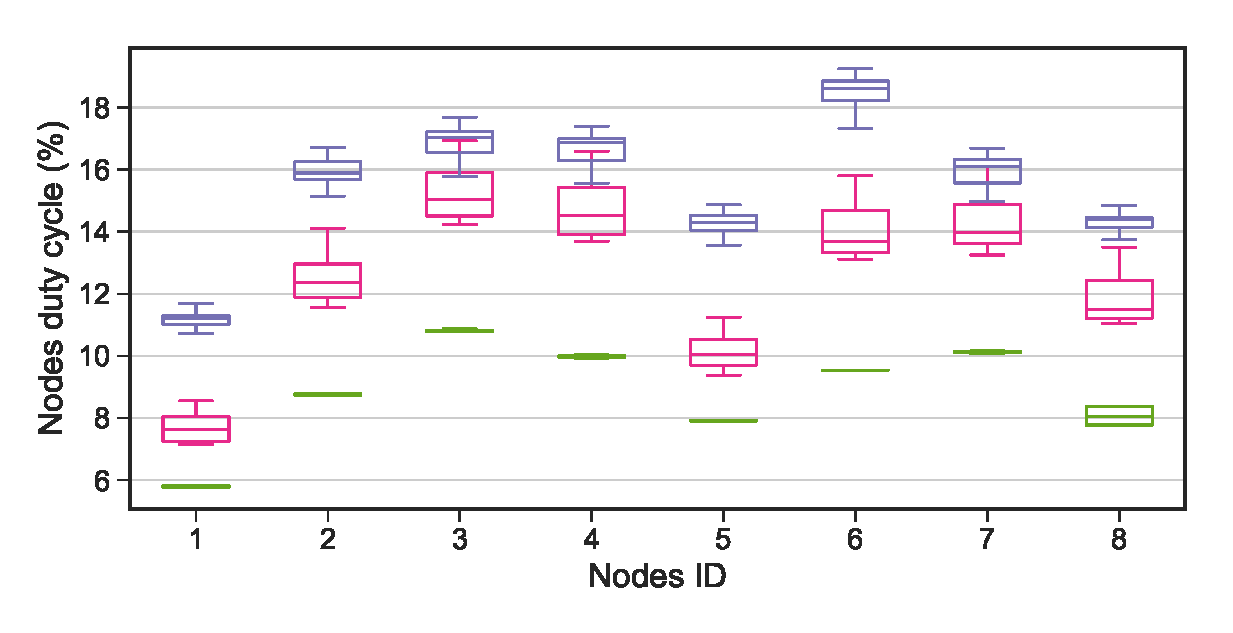
\includegraphics[width=\textwidth]{figures/natural_light_nodes_duty_cycles}
				\caption{\todo{correct the figures} RF}
		\end{subfigure}
		\caption{nodes's duty cycles are different for different energy conditions and different energy sources.}
		\label{fig:pwrCIS}
\end{figure} 

\paragraph{Implicit distribution of nodes' on-times}
Figure~\ref{fig:pwrCIS} shows the availability of \sys{}s when they are powered by different energy source and for a different number of intermittent nodes. We see that (i) the energy sources (sunlight, artificial light, and RF) power the \sys intermittently, (ii) the \sys availability increases with number of nodes, and (iii) this addition is proportional to the \sys off-time. 

The dashed lines represent Equation~\ref{eq:cisModel} expectation about the \sys availability for certain power cycles (10\% for the RF powered system, and 15\% for the light powered one). By comparing these lines to the measured ones we can conclude that these energy sources provide sufficient randomness to cause each node to have a slightly different power cycle which, in turn, causes their uptimes to be uniformly distributed in time.  


\subsection{Power States}
\label{sec:power_state}
A \sys can experience a wide range of ambient power intensities. For example, a solar-powered \sys may harvest no energy at night, modest energy from artificial light, and abundant energy from direct sunlight.  Generally, we can identify four different \sys powering states: 
\begin{itemize}
		\item \textit{Targeted power state}---These are the powering conditions that the \sys is designed for. In these  conditions, the \sys should work intermittently and have sufficiently randomized power cycles to uniformly distribute its intermittent nodes on-times and meet the desired availability percentage (Figure~\ref{fig:cisModel}). In general, the targeted powering conditions should be near worst energy harvesting conditions to ensure that the system is properly functioning for the majority of the time.
		\item \textit{Under-targeted power state}---Ultimately, the ambient energy is an uncontrollable power source, and it is not hard to imagine scenarios where a \sys will be under-powered or even comes to complete and long power down (for example, a solar \sys will come to a perpetual power down in the darkness). In general, for under-targeted energy conditions, the \sys behavior can be considered as undefined.
%
\begin{figure}
		\centering
		\includegraphics[width=\columnwidth]{figures/hibernating_power_state}
		\caption{\fullsys is in a hibernating power state when the energy harvesting rate approximates the energy consumption rate at the sleeping (or low-power) mode. In this state, the intermittent nodes lose the randomization in their power cycles. Thus, all the nodes capture the same event and power down shortly after missing the subsequent ones. Consequently, the \sys senses intermittently and does not take advantage of its redundant intermittent nodes to approach continuous sensing.}
		\label{fig:noRand}
\end{figure} 
%
		\item \label{it:hibernating} \textit{Hibernating power state}---In event-based sensing scenarios, the intermittent nodes of a \sys sleep in low-power mode waiting for an external event to wake them up. If the energy conditions are relatively higher than the targeted conditions, the nodes may not die and sustain their sleeping power consumption. This will cause them to synchronize their wake-ups on the first incoming event and their power down as the event capturing process depletes their energy buffers quickly. Consequently, the \sys may miss the next incoming events (specially if the events happens to arrive in bursts) causing it to sense intermittently instead of continuously, see Figure~\ref{fig:noRand}. 
		\item \label{it:continuous} \textit{Continuous power state}---Under direct mid-noon sun even a tiny solar panel can continuously power a sensor. In such conditions, the \sys will sense continuously without the need for randomization. Therefore, the job of a single node will be repeated $N$ times, and instead of sending a single message to a battery-powered or tethered sink---to push the data to the internet---$N$ identical messages will be sent which waste a lot of energy. 
				
\end{itemize}
%
\begin{figure}
		\centering
		\includegraphics[width=\columnwidth]{figures/randomized_response}
		\caption{Randomized response helps in mitigating the hibernate-power-state problem. Also, it reduces the number of duplicated captured events when the \sys is overpowered. However, effective randomization strategy must be energy aware.}
		\label{fig:rand}
\end{figure} 

The inefficiencies highlighted in the hibernating and continuous power states can be mitigated by enforcing randomization on the response of intermittent nodes (Figure~\ref{fig:rand}): when a node is woken up by an external event it responds to that event with a certain probability. However, if the randomized response is enforced all the time, then the \sys will have a lower probability of catching events during the targeted energy conditions. Therefore, the \sys has to distinguish between the targeted and above-targeted energy conditions and randomize its response only during the hibernating and continuous power states. 


Choosing a fix response probability is an inefficient way of dealing with the over-powering problem as the number of active intermittent nodes at a given moment is a function of the total number of intermittent nodes and the power intensity at that time. Therefore, efficient randomization requires intermittent nodes to estimate the number of active nodes at the moment of an external event arrival (which is discuss it next) and respond proportionally.


\subsection{Intermittent Timing}
\label{subsec:interTimer}
%
\begin{figure}[t]
		\centering
		\includegraphics[width=\columnwidth]{figures/softwareClock}
		\caption{....}
		\label{fig:softwareClock}
\end{figure} 
%

Timing is a key building block of sensing systems. However, it is missing on intermittent nodes unless an additional dedicated timer circuit is added to them~\cite{hester2017timely}. Here we would like to propose an alternative way that does not require additional timer hardware. Obviously, the on-time of an intermittent node can be measured using the microcontroller's built-in timers. However, the difficulty is \textit{how an intermittent node can time its own off-time?}. Actually, answering this question does not only enable timing on intermittent devices but also enables them to estimate the richness of the ambient energy. 

\paragraph{Timing the death} 
Algorithm~\ref{algo:offTime} shows how a node can estimate its off-time. The basic idea is that a node measures its on-time while harvesting (Line~\ref{lin:ontime}) and compares it to the time required to drain the super capacitor without charging. The additional on-time $\Delta{t}$ is the result of the energy accumulated while executing. (Line~\ref{lin:deltat}). By assuming a relatively stable charging rate, a node can calculate how long it will be off charging (Line~\ref{lin:ehar}-\ref{lin:offtime}). Obviously, in order for the time estimation to be correct, the reference time and the on-time measurement must be done with same load ($a$). %\textcolor{red}{\bf Stephan: not sure what is meant here with "with same load"??/}
% off-time estimation 
\begin{algorithm}[t]
	\captionof{algorithm}{off-time estimation}
    \label{algo:offTime}
    \small
    \begin{algorithmic}[1]
		\State \Call{$f_\text{reboot}$}{$u$} $= u{+}{+}$ \Comment{power reboot counter}
		\State $i \leftarrow $ \Call{$f_\text{reboot}$}{$i$} \Comment{$i$ is a persistent variable}
		\State $E_\text{buf}$ \Comment{Size of energy buffer}
		\State $t_a$ \Comment{time of discharging $E_\text{buf}$ at load $a$, no harvesting}
		\State$ t_{i} \leftarrow x $ \Comment{timing every $x$ power cycles}
		%
		\If{$(i\mod t_{i})=0$}
		    \State $i=0$
			\State \Call{$f_\text{load}$}{$a$} \Comment{set node load to $a$ }
			\State \label{lin:ontime} $t_\text{on} \leftarrow$ \Call{$t_\text{pers}$}{\null} \Comment{persistent infinite loop}
		\EndIf
		\If{$i=0$}
			\State \label{lin:deltat}$\Delta{t} = t_\text{on}-t_a$  \Comment{time difference due to charging}
			\State \label{lin:ehar}$E_\text{har} \leftarrow (E_\text{buf}\div t_a)\times\Delta{t}$ \Comment{harvested energy}
			\State $P_\text{in} \leftarrow E_\text{har}\div{t_\text{on}}$ \Comment{incoming power}
			\State \label{lin:offtime}$t_\text{off} \leftarrow E_\text{buf}\div P_\text{in}$
		\EndIf
	\end{algorithmic}
\end{algorithm}

\subsection{Nodes overlapping}
\begin{figure}[t]
		\centering
		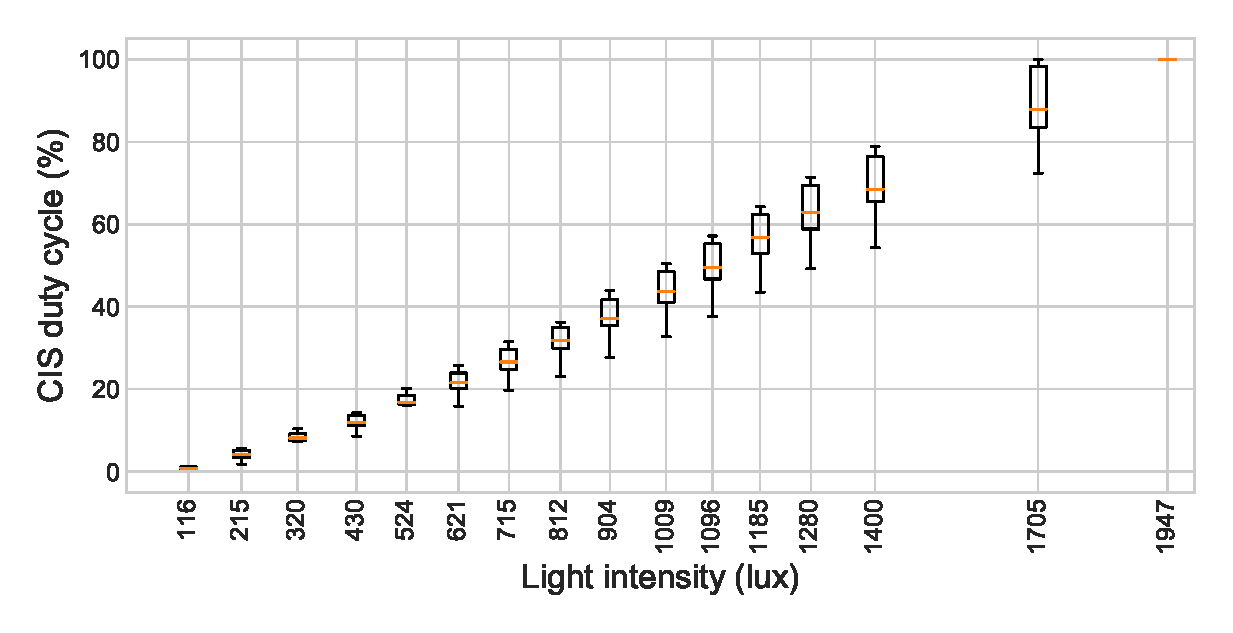
\includegraphics[width=\columnwidth]{figures/cis_dutyCycle.eps}
		\caption{The average duty cycles of eight intermittently powered nodes for different light intensity. In general, an individual node's duty cycle is a good indicator of the average duty cycle of its \sys.}
		\label{fig:cis_nodes_dutyCycle}
\end{figure} 

\begin{table}
		\centering
		\caption{Measuring intermittent nodes overlapping of a \sys of 8 intermittent nodes for different light intensities.}
		\begin{tabular}{lll}
				\hline
				light intensity (lux) & mean & std    \\
				\hline
				300	                  & 1.01 & 0.85   \\
				500                   & 1.63 & 0.98   \\
				800                   & 2.88 & 1.50   \\
				1200                  & 5.05 & 1.08   \\
				\hline
		\end{tabular}
		\label{tab:clusters}
\end{table}


In order for a node to estimate the number of active nodes at a given moment, first, it has to know the total number of nodes ($N$) in its \sys, which we assume to be known to the nodes before deployment. Second, this analysis is built on the observation that a node's on-time is a good indicator about the on-times of other nodes in the \sys, see Figure~\ref{fig:cis_nodes_dutyCycle}. A node can measure its on-time $t_\text{on}$ and off-time $t_\text{off}$ using  Algorithm~\ref{algo:offTime} (or an external dedicated timer~\cite{hester2017timely}). Then, it can estimate the maximum time span ($t_\text{max}$) of its \sys, which is the total duration of the nodes' on-times when they are aligned next to each other, as follows
\begin{equation}
t_\text{max} = N\times t_\text{on}.
		\label{eq:max_time}
\end{equation}
Then, from Equation~\ref{eq:cisModel}, the node calculates the \sys expected on-time ($t_\text{on}(N)$). As we argued in Section~\ref{subSec:availability}, nodes on-times are uniformly distributed over the \sys power cycle. Thus, the overlapping on-time is also uniformly distributed over the \sys on-time. Then, a node can calculate the average number of active intermittent nodes $n_\text{active}$ using the following formula,
\begin{equation}
	n_\text{active} = t_\text{max} \div t_\text{on}(N).
	\label{eq:active}
\end{equation}
and choose the proper randomization factor. If a second event, however, happens shortly after the first one, a node needs to update $N$ as follows, 
$$
N = N - n_\text{active}-1
$$
the $-1$ is because the node itself decided not to react on the first event. 

Table~\ref{tab:clusters} shows the average number of overlaps of an 8-nodes \sys for different light intensities. These measurements validate that nodes overlapping time is uniformly distributed over the \sys on-time. For example, at $\SI{1200}{lux}$ an individual node of our \sys has a duty cycle of $\approx$\,62\%. If we multiply it by the number of nodes (Equation~\ref{eq:max_time}) we get about 500\%. Figure~\ref{fig:cisModel} indicates that a \sys with eight nodes of duty cycles above 50\% has near 100\% availability. From equation~\ref{eq:active}, we find that the expected number of clustered nodes is 5 which is what Table~\ref{tab:clusters} also shows. 



%\section{Distributed Intermittent System}
\section{Batteryless Distributed Microphone}
\label{sec:disMic}
\begin{figure}
	\centering
	\includegraphics[width=\columnwidth]{figures/cis}
	\caption{\fullCIM: an instant of a \fullsys. \cim features a power failure immune word recognizer. Once a word is recorded, the word's spectral features extraction begins. The resulting features vector is compared against previously-stored words' templates for recognition. The comparison using a liner distance matching algorithm}
	\label{fig:cis}
\end{figure}

We have developed a prototype of a \fullcim (\cim): an instant of a \fullsys. The \cim consists of eight batteryless intermittent nodes. Each node is capable of performing isolated words recognition. 

The reason behind developing a \cim is threefold: (i) voice is a natural and convenient way for human to interact with miniaturized devices; (ii) demonstrating \textit{the world's first} batteryless intermittently-powered command recognizer, which shades light on the potential of batteryless intermittent systems; and (iii) facilitating testing with different sensing strategies and different type of external events arrival (i.e., regular  or burst). 


% Moreover, we believe that a \cim can facilitate direct human-to-human or human-to-objects communication. Imagine that a \cim based system is deployed in a play ground, embedded in ground and other objects. You want to call your child, and a \cim based system is embedded in your shirt and his shirt. You say his name and the \cim picks up the word and scatter it over light---\cite{marco}  demonstrates the feasibility of scattering sunlight to communicate between two nodes that are up to 60\,m apart. The scattered signal will be relied on other \cim nodes until the receiving node on his shirt receives the message and notify him, daddy is calling. 

\subsection{Hardware}
\label{sec:hardware}
A \cim node consists of thee main parts: a microphone, a microcontroller, and a harvester. MSP430RF5994~\cite{ti_msp430_website}, an ultra-low-power microcontroller, is used for data acquisition and processing. This microcontroller has a 16-bit RISC processor running on 1 MHz, 8KB of SRAM (volatile), 256KB of FRAM (non-volatile), and a 12-bit analog to digital converter (ADC). It also features a Low Energy Accelerator (LEA), which offloads the main CPU for specific operations, such as FFT. For recording we use the PMM-3738-VM1010-R piezoelectric MEMS microphone, which features Wake on Sound and ZeroPower listening technologies \cite{microphone}, allowing both the microcontroller and the microphone to sleep in a low-power mode until a sound wave is detected.
The microcontroller and microphone are powered by a BQ25570 solar power harvester~\cite{BQ25570EVM-206_website} connected to an IXYS SLMD121H04L solar cell~\cite{SLMD121H04L_website} and a super-capacitor of 470 \si{\micro F}. For debugging we used the Saleae logic analyzer~\cite{saleae}.

\subsection{System Description}
The \cim has a power interrupts immune command recognizer. The recognizer is capable of recognizing isolated-word type of speech. 
The main parts of the recognizer are illustrated in Figure~\ref{fig:cis} and explained below:

\subsubsection{Data acquisition}
The \textit{Wake-on-Sound} feature of the microphone triggers the data acquisition process once the energy level in the sound signal crosses a certain level. The ADC, then, samples the output of the microphone at 8\,kHz. This sampling rate is sufficient to cover most of the frequency range of the human voice. To determine the end of the recording we relied on the characteristics of the targeted vocabulary. In particular, we identified experimentally the minimum effective recording length, which is 
%happened be 
285\,ms for the chosen set of words. By exploiting the Wake-on-Sound feature and using the minimum effective recording length, we eliminate the need for an endpoint detection algorithm, greatly improving the processing time and system efficiency from the energy perspective.


\subsubsection{Feature Extraction}
Once a recording has finished, framing and data processing begin. \cim divides the digitized signal into non-overlapping frames of 256 samples ($\approx$ 33 milliseconds). This size is beneficial for doing a Fast Fourier Transform and short enough for the voice-features to be considered constant inside a frame.

To extract the spectral features of a frame, \cim divides the frequency of interest into 12 bands (as in~\cite{hopper1992}). The first five bands has a bandwidth of 200\,Hz. The next three has a bandwidth of 300\,Hz which is followed by two bands of 500\,Hz. Finally, the last two bands has a 600\,Hz bandwidth. This division is motivated by how the energy is concentrated in human speech~\cite{hopper1992}. Then, \cim computes the 256-point Fast Fourier Transform for each frame. The resulting feature vector contains the amount of energy concentrated in each frequency band defined earlier. This feature vector forms the basis for the words identifying process once it is normalized.

We normalize the feature vectors to minimize detection errors that result from differences in the amplitude of the speech input. To normalize a feature vector, \cim computes the binary logarithm of each entry of that vector. 
Then it computes the mean of the resulting vector. Finally, it subtracts the computed mean from each entry of the resulting vector. This is summarized in the following equation: 
\begin{equation}
    f_i = \log(\hat{f}_i) - \frac{\sum\limits^S_{i=1}\log(\hat{f}_i)}{S},
\end{equation}
where $f_i$ is the normalized output for the $i^{\text{\tiny th}}$ spectral band of a feature vector, $\hat{f}_i$ is the energy in the $i^{\text{\tiny th}}$ spectral band of the frame, and $S$ is the number of spectral bands (12 in our case). 

\subsubsection{Feature Matching}
% %
% \begin{figure}
% \centering
% 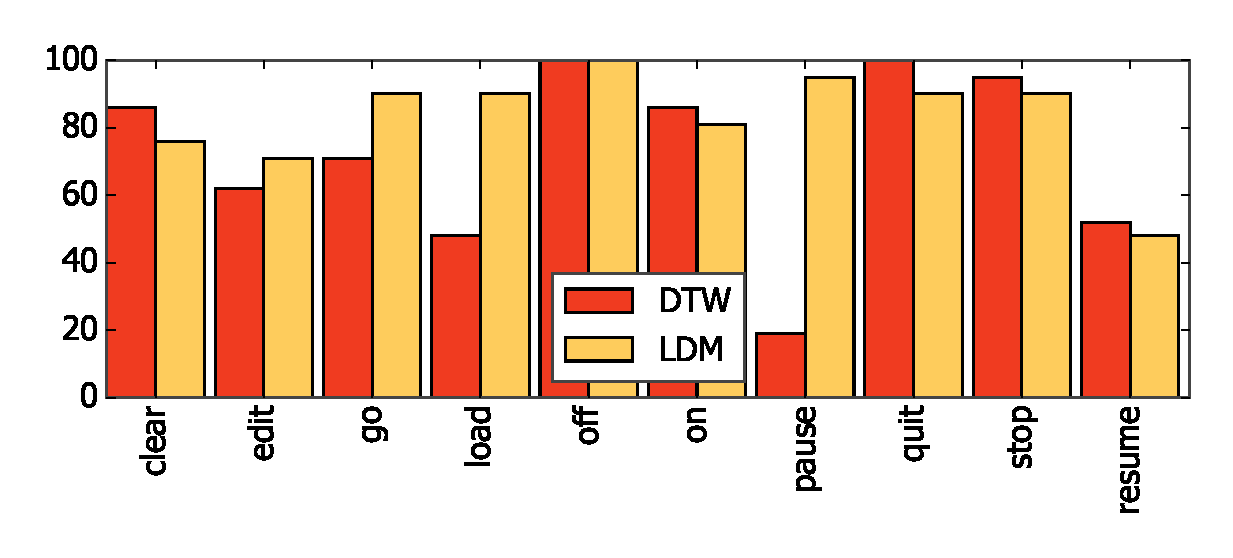
\includegraphics[width=\linewidth]{figures/DTWvsLDM}
% \caption{Recognition accuracy for linear matching and DTW when using 9 frames as the recording length.}
% \label{fig:DTWvsLDM}
% \end{figure}
% %
\begin{table}
	\centering
	\caption{Profiling of features matching algorithms: Dynamic Time Warping (DTW) and Linear Distance Matching (LDM)}
	\label{tab:profiling}
	\begin{tabular}{lll} \hline
	Section & LDM (ms) & DTW (ms) \\\hline
	Recording & 285  & 285 \\
	Feature extraction & 501 & 501 \\
	Feature matching &  99 & 1251 \\\hline
	Total & 885 & 2037 \\\hline
	\end{tabular}
\end{table}
%
Feature matching is achieved by computing the distances between the normalized feature vectors of the recorded word and the feature vectors of the words stored during the training phase (templates). 
\cim computes the squared Euclidean distance between vectors as follows:
\begin{equation}
	 	d_j = \sum\limits^S_{i=1} (f_{s,i} - f_{r,i})^2,
    \label{eq:frame_dist}
\end{equation}
where $d_j$ is the distance between the $j^{\text{\tiny th}}$ stored and recorded vectors. $f_{s,i}$ is the normalized output of the $i^{\text{\tiny th}}$ spectral band of a stored vector, $f_{r,i}$ is the normalized output of the $i^{\text{\tiny th}}$ spectral band of a recorded vector. 
The total distance between two words is calculated as follows:
\begin{equation}
		D_k = \sum\limits^{l}_{j=1} d(j)
\end{equation}
where $D_k$ is the distance between the $k^{\text{\tiny th}}$ stored word and the recorded word, and $l$ is the recording length measured in frames.

Once the recorded word has been compared to all \cim template words, the template with the smallest distance to the recorded word is considered the correct word. However, if the smallest distance is bigger the garbage threshold which we experimentally set, then the \cim will return "undefined word". 

It should be emphasized that in linear distance matching (LDM) the feature vectors of two words are compared successively, not accounting for differences in pronunciation speed. This is sufficient for our case as we are targeting isolated words and speaker dependent speech recognition type. We also implemented the Dynamic Time Warping algorithm which better handles the difference in the speed of speech. However, it is slower than the linear matching algorithm  (Table~\ref{tab:profiling}) and the detection accuracy was comparable in our case.% (Figure~\ref{fig:DTWvsLDM}). 

\subsubsection{Power Failure Protection}
In order to preserve the progress state and to protect \cim data against randomly timed power failures, we manually split \cim program into 19 atomic regions. We ensured the each of these regions requires less energy then what the energy buffer can provide with a single charge. The program progress state is saved in the non-volatile memory (FRAM) on the transition between these regions. This prevents the program from falling back to its starting point (\texttt{main()}) after each power failure. Data in the non-volatile memory with Write-After-Read dependency is double buffered to ensure data integrity when the power supply is interrupted. 

\subsection{Code profiling}
The entire command recognition software was written in the {\tt C} programming language. The total program consists of 973 lines of code, excluding the FFT function from the Texas Instrument DSP library. See Table~\ref{tab:code_stats} for more information.

The memory footprint on the microcontroller is 20,064 bytes of FRAM and 1,134 bytes of SRAM. Execution times are shown in Table~\ref{tab:profiling}.

The power usage of a node differs according to it's activity. When a node is waiting for a voice event, it is in low-power mode. When data needs to be processed or recorded it is in active mode. When recording, the microphone and ADC consume additional power. The power consumption rates are determined by measuring the current with a Monsoon power monitor~\cite{monsoon} and shown in Table~\ref{tab:power_usage}.


\begin{table}
	\centering
	\caption{Code statistics: lines of code}
	\label{tab:code_stats}
	%Compiled without optimization flags:
	\begin{tabular}{lrrrr} \hline
		Language & Files & Blank & Comment & Code \\\hline
		C & 7 & 264 & 173 & 736 \\
		C/C++ Header & 8 & 62 & 40 & 237 \\\hline
		Total &  15 & 326 & 213 & 973 \\\hline
	\end{tabular}
\end{table}

\begin{table}
	\centering
	\caption{Power usage.}
	\label{tab:power_usage}
	%Compiled without optimization flags:
	\begin{tabular}{lrrr}\hline
	Section & Current (\si{\micro A}) & Voltage (V) &  Power (\si{\micro W}) \\\hline
	Sleeping & 64 $\pm$20 & 2.008 & 128 $\pm$40 \\
	Recording & 423 $\pm$20  & 2.008 &  849 $\pm$40\\
	Processing &  282 $\pm$20 & 2.008& 566 $\pm$40 \\\hline
	\end{tabular}
\end{table}

\section{Evaluation}
\label{sec:evaluation}
\begin{table}[H]
\centering
\caption{Testing set}
\label{tab:words}
\begin{tabular}{lllll}
\hline
on    & off  & stop & clear & load   \\
go & pause & resume & edit  & quit  \\  
\hline  
\end{tabular}
\end{table}

\subsection{Effective recording length}
\label{subsec:rec_length}
%
\begin{figure}
	\centering
	\includegraphics[width=\linewidth]{"figures/linear_multi"}
	\caption{Recognition accuracy versus the recording length (in frames), while using multiple recordings per word for testing. Used feature matching method: linear.}
	\label{fig:multi}
\end{figure}
%
Since our target hardware has extremely limited resources, the first experiment targets the minimum effective recoding length without significant accuracy loss. 

For this experiment a single microcontroller running on continuous power is used. Each word from Table~\ref{tab:words} was recorded on a PC 20 times. The features---normalized FFT-based values---of the first recording are saved in the microcontroller's persistent memory as a signature to perform the feature matching, during the testing. the rest of the recording are used for conducting the experiment.   

Figure~\ref{fig:multi} shows words recognition accuracy when the 19 recordings of each word are played back from the PC speaker. We can concluded that recording beyond \textit{nine frames} do not increase the recognition accuracy; therefore, nine frames recording length is chosen for the rest of the experiments. 

\subsection{Comparison of feature matching methods}
%
\begin{figure}
\centering
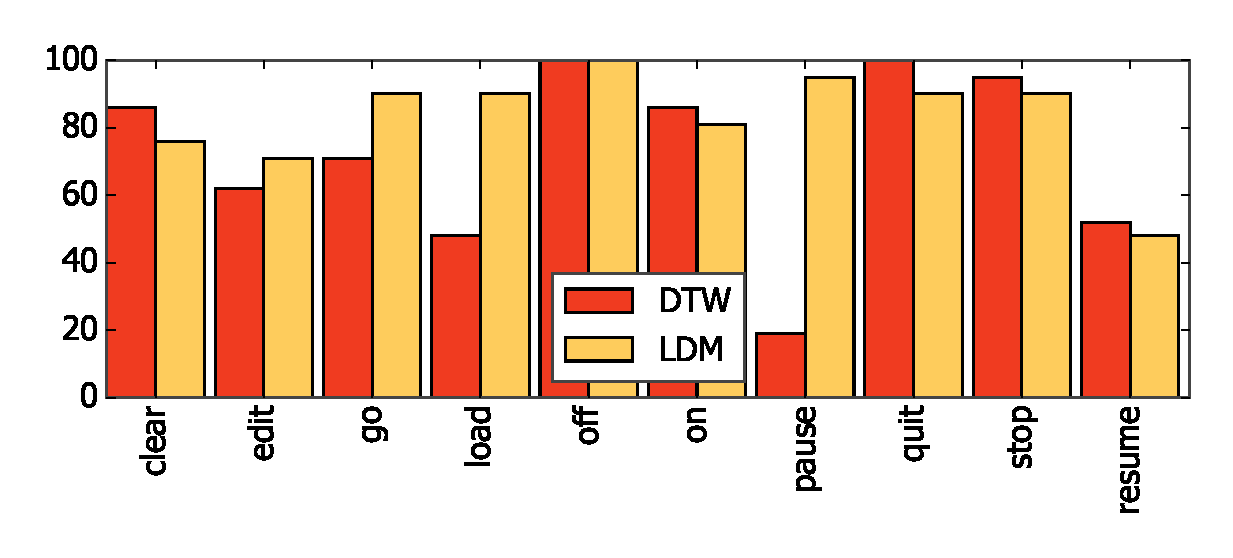
\includegraphics[width=\linewidth]{figures/DTWvsLDM}
\caption{Recognition accuracy for linear matching and DTW when using 9 frames as the recording length.}
\label{fig:DTWvsLDM}
\end{figure}
%
\begin{table}
	\centering
	\caption{Profiling of features matching algorithms: Dynamic Time Warping (DTW) and Linear Distance Matching (LDM)}
	\label{tab:profiling}
	$
	\begin{tabular}{lll}\hline
	Section & Linear (ms) & DTW (ms) \\\hline
	Recording & 285.9  & 285.9 \\
	Feature extraction & 501.9 & 501.9 \\
	Feature matching &  99.4 & 1251 \\\hline
	Total & 887.2 & \\\hline
	\end{tabular}
	$
\end{table}
%
We implemented two algorithms for voice features matching, Dynamic Time Warping (DTW) and Linear Distance Matching (LDM). Due to the microphone wake-on-sound feature and the fixed recording length, DTW did not outperform LDM as Figure~\ref{fig:DTWvsLDM} shows. Moreover, DTW takes more time to process that data as Table~\ref{tab:profiling} shows. Therefore, LDM algorithm is used in future experiments.

\subsection{ Intermittent microphone availability}
%

\begin{figure}
\centering
\includegraphics[width=\linewidth]{figures/word_freq}
\caption{The effect of the time between consecutive words on the availability: the percentage of words that is processed by the command recognizer. \todo{Add correct recognition as stacked bar?}}
\label{fig:word_freq}
\end{figure}
%
\begin{table}
	\centering
	\caption{The mean and standard deviation of the parameters that were used to simulate intermittent execution. Here $t_{on}$ is the time the device is on while recording or processing, $t_{off}$ is the time the device is charging and $t_{sleep}$ is the time the device is sleeping while waiting on sound input.}
	\label{tab:simparams}
$
\begin{array}{lll}\hline
\text{Parameter} & \mu \text{ (ms)} & \sigma \text{ (ms)} \\\hline
%t_{rec} & 295 & 0 \\
t_{on} &  590 & 17.7 \\
t_{off} & 5310 & 154 \\
t_{sleep} &  22420 & 652 \\\hline
\end{array}
$
\end{table}
%
This experiment shows the effect of intermittent power supply on a microphone availability \todo{and recognition accuracy} for different command (or word) repetition speed. Each word (from Table~\ref{tab:words}) was played back 20 times with intra-words-playing time ranges from 1 to 10 seconds. 

For the experiment we chose to simulate the intermittent power supply, based on a real measurement, to ensure environment consistency across different words.
In particular, we measured the $t_{on}$; used an on/off ratio of $10\%$ to simulate harsh harvesting conditions~\cite{mementos, harvOS,lucia}; and calculated the $t_{sleep}$ based on the micro controller specification~\cite{datasheet} (Table~\ref{tab:simparams}).     

The obvious observation from Figure~\ref{fig:word_freq} is that intermittency has a great impact on the command recognizer availability. However, a less obvious, but important, observation is that the correlation between the on/off cycle and the command repetition speed has also great impact as the bars labeled with 5 and 6 from Figure~\ref{fig:word_freq} indicate. 







\section{Background}
\label{sec:background}
Here a minimal amount of background information is presented to facilitate clarifying the technical sections of the paper. 

\subsection{Energy-harvesting Devices}

%1. why \textit{small form factors EH sensor nodes}\\
Small sensors are less intrusive devices, and therefore, many applications prefer them on the bigger ones 
% (imagine the difference in the implications of embedding a sensor of the size of 2 AAA batteries and a sensor of a few cubic millimeters in volume in a shoe for step counting).  
%
Long sensors lifetime is also desirable. However, long sensors lifetime and small form factors are conflict goals.
% 2. classify EH with continuous power and tiny EH with intermittent power \\
For example, rechargeable batteries paired with energy harvesters can continuously power sensor nodes for relatively long time. But, rechargeable batteries inherent normal batteries drawbacks including increasing the size and limiting the sensor lifetime (although much longer) as rechargeable batteries typically wear out after a few hundreds charging cycles~\cite{}.
%
However, if an application's requirements put hard constraints on the size of the sensors, then removing the batteries is one of the first options to be considered. 
Battery-less energy-harvesting sensors operate intermittently. They charge a small capacitor to ensure uninterrupted operations for a minimum certain duration. Once, the capacitor has been depleted, the sensor powers down, letting the energy-harvester to accumulate energy again. 
%
Intermittent operation raises many challenges such as how to enable applications to span their execution over power failure~\cite{}, and how to enable timeliness operations when the durations of the device power-downs are indeterminate~\cite{}.
%
Big capacitors may allow longer operational periods of time, but they also need more time to charge. 
In order for a capacitor to charge, the input voltage must be higher than the accumulated voltage in the capacitor. 
This phenomena makes charging big capacitors using tiny energy harvester less efficient~\cite{}. 
boosting ambient energy using an energy-conditioning circuit is possible on the expense of device complexity, form factor, energy consumption, and cost. 

\subsection {Speech types}
%
Speech recognition algorithms can be classified based on the type of speech that they can recognize into \textit{spontaneous speech, continuous speech, connected word,} and \textit{isolated word}~\cite{gaikwad2010review}.
Systems with \textit{continuous} or \textit{spontaneous speech} recognition are the closest to natural speech, but are the most difficult to create because they need special methods to detect words boundaries~\cite{gaikwad2010review}. This is less the case for the \textit{connected word} type, where a minimum pause between the words is required.
 The type with the least complexity is the \textit{isolated word} type. It requires a period of silence on both sides of a spoken word and accepts only single words. 
 
Voice is a natural way for the human to interact with small devices. However,
implementing speech recognition on resources---memory, computation power, and energy---limited platforms is challenging, to say the least. Therefore, we attempt to recognize, with our command recognizer prototype, the simplest type of speech, isolated words. 

\section{Related Work}
\label{sec:relatedWork}
Recent advances in ultra-low-power microcontrollers along with the development of energy harvesters have enabled the creation of stand-alone battery-free sensors. These sensors operate intermittently because the power that they harvest is
weak and volatile.

\subsection{Energy-harvesting systems}
Energy harvesters have the potential to power devices indefinitely as they collect energy from perpetual energy sources. Sunlight, vibration, and radio frequency (RF) waves are examples of such energy sources. The power harvested from these sources vary wildly, for example, RF harvestable power ranges from
\si{\nano\watt}-scale when harvested from ambient signals to \si{\uW}-scale when collected from a dedicated RF signal emitter, and solar power varies from tens of \si{\uW} to tens of \si{\mW} when it is harvested by a solar panel of a few \si{\cm^2} illumination surface~\cite{lucia2017intermittent,rao2017ambient}.

Many battery-less EH platforms have been proposed. Some of them
rely on dedicated external energy sources such as WISP -and its variants-, a
general wireless sensing and identification
platform~\cite{smith2006wirelessly,zhao2015nfc,zhang2011moo}; WISPcam,  an
RF-powered camera~\cite{naderiparizi2015wispcam} and, the battery-free
cellphone~\cite{talla2017battery}. Others, harvest from ambient sources such as
the ambient backscatter tag~\cite{liu2013ambient}, and the solar-powered
tag~\cite{majid2019multi}. Platforms that facilitate the development of
battery-less EH systems have also been proposed. For instance,
Flicker~\cite{hester2017flicker}, a prototyping platform for battery-less devices; EDB~\cite{colin2016energy} an energy-interference-free debugger for intermittent devices;  and Capybara~\cite{colin2018reconfigurable}, a re-configurable energy storage architecture for EH devices.

However, \emph{there is no EH platform that considers the abstraction of many intermittent sensors (or nodes) and exploits the statistical energy harvesting differences between them to provide reliable sensing}.
% The paper is the first that considers the abstraction of a group of intermittent nodes and investigates the emerging collective duty cycle of the system. 
%experience. 

\subsection{Intermittent execution}
% What is the problem that requires intermittent execution
Intermittent execution models enable applications to progress despite frequent
power failures~\cite{van2016intermittent,colin2016chain,lucia2015simpler,bhatti2017harvos,gobieski2019intelligence}. To this end, they decompose an application into several small pieces and save the state of the computation on the transitions between these code segments. Therefore, intermittent applications do not return to the beginning of the program (i.e., \texttt{main()}) after each power failure.
%(in contrast to  applications that assume continuous power).
Instead, they resume execution from the last successfully saved progress state.   

% Sleep not to die 
% Intermittent systems are regarded as the successor of energy-aware systems. Dewdrop~\cite{buettner2011dewdrop} is an energy-aware runtime for (Computational) RFIDs such as WISP. Before executing a task, it goes into low-power mode until sufficient energy is accumulated. QuarkOS~\cite{zhang2013quarkos} divides the given task (i.e., sending a message) into small segments and sleeps after finishing a segment for energy recharge. However, these systems are not power disruption tolerant. In other words, if a system could not sustain the energy consumption of low-power mode and powers down, then all the computation progress will be lost. 

% checkpointing 
Mementos~\cite{ransford2011mementos} proposed a volatile memory \emph{checkpoint-based} approach to enable long-running applications on intermittently powered devices. DINO~\cite{dino} enables safe non-volatile memory access despite power failures. Chain~\cite{colin2016chain} minimizes the amount of data needed to be protected by introducing the concepts of \emph{atomic tasks and data-channels}. Hibernus~\cite{balsamo2014hibernus,balsamo2016hibernus++} measures the voltage level in the energy buffer to reduce the number of checkpoints per power cycle. Ratchet~\cite{van2016intermittent} uses compiler analysis to eliminate the need for programmer intervention or hardware support. HarvOS~\cite{bhatti2017harvos} uses both compiler and hardware support to optimize checkpoint placement and energy consumption. Mayfly~\cite{hester2017timely} enables time-aware intermittent computing. InK~\cite{yildirim2018ink} introduces event-driven intermittent execution.  
\emph{For our prototype implementation we adopt a power failure protection approach similar to that of DINO~\cite{dino}, see Section~\ref{sec:software}.}

\subsection{Explicit duty-cycle desynchronization}% in Sensor Networks}
Explicit duty-cycle desynchronization has been proposed in the sensor network literature~\cite{degesys2007desync,giusti2007decentralized,zheng2013survey}. 
These (biologically-inspired) algorithms, however, cannot be applied to desynchronize intermittently-powered nodes as they assume that nodes (i) are able to listen to other nodes, and (ii) can maintain a notion of global time (slots). Listening is expensive, and keeping track of time is difficult at best when nodes can power down at random moments. We therefor adopt a best-effort approach.

\subsection{Speech recognition}
%  Speech recognition consists of several steps. The basic steps are:
% \textit{Speech recording and signal digitization}---a microphone records the sound waves and an ADC converts the microphone signal into a digital signal. A sampling rate of about 8 kHz is required to capture the frequencies of a human voice (100-4000Hz \cite{Bernal-Ruiz2005MicrocontrollerSystems}). \textit{Framing}---after that the digitized signal is divided into blocks of usually 10-30 ms~\cite{gaikwad2010review,delaney2002low,delaney2005energy} called frames. \textit{Features extraction}---for each frame a feature vector is extracted containing all the relevant acoustic information. \textit{Feature matching}---finally the extracted features are matched against features known to the recognizer. 

The speech recognition problem has been tackled from many angles and has experienced many breakthroughs. For example, the dynamic time warping (DTW) algorithm enables matching voice signals with different speed (or time) \cite{vintsyuk1968speech}. 
Approaches based on Hidden Markov Models showed much better performance than DTW-based ones~\cite{jelinek1997statistical}. Hence, they became the standard techniques for general-purpose speech recognition until artificial intelligent algorithms~\cite{hinton2012deep} outperform them. 
% Furthermore, many specialized hardware architectures for speech recognition have been proposed to, for instance, reduce energy consumption \cite{price2018low,price20156}. 

% The evolvement of the speech recognition algorithms has enabled them to recognize more complicated type of speech. 
% From a recognition algorithm perspective the speech can be classified
% Speech recognition algorithms can be classified based on the type of speech that they can recognize 
From a recognition complexity standpoint, we can classify the speech into \textit{spontaneous speech, continuous speech, connected word,} and \textit{isolated word}~\cite{gaikwad2010review}.
The \textit{continuous} and \textit{spontaneous speech} are the closest to natural speech, but they are the most difficult to recognize because they need special methods to detect words boundaries~\cite{gaikwad2010review}. This is less the case for the \textit{connected word} type, where a minimum pause between the words is required. The type with the least complexity is the \textit{isolated word}, as it requires a period of silence on both sides of a spoken word. 
 
% Voice is a natural way for the human to interact with small devices. However, 
Speech recognition on resources---memory, computation power, and energy---limited platforms is challenging, to say the least. Therefore, \emph{our command recognizer targets isolated-word type of speech}. 





















\section{Discussion and Future Work}
\label{sec:discussion}

\section{Conclusion}
This paper addresses the availability problem of intermittent sensors
that fail to capture (and process) events while charging their energy
buffer.  As the power to drive a node is much higher than what can be
harvested from ambient sources, the chance of capturing an event can
be as low as just 8\% (sunlight) and 4\% (RF) (cf.\ the duty cycles
reported in Figure~\ref{fig:cis_nodes_dutyCycle}). To address this problem of missing
most events we presented the \fullcis (\cis),
which is the abstraction of a group of intermittently-powered sensors,
whose collective duty cycle (on-time) can approach the desired 100\%
availability.  The inherent differences in the powering subsystem of
intermittent sensors result in (slight) differences in the sensor nodes'
power cycles causing the nodes' on-times to be uniformly distributed. This
implies that simply selecting the right number of nodes is all that
is required. To this end we have modeled the (effective) availability
of a \cis and validated its accuracy against data collected on real
hardware.

Experimentation with an 8-node prototype \cis, a basic voice-control
application recognizing up to 4-word commands, showed that the inherent
randomization in the power cycles can easily be disrupted. In case the
ambient power exceeds the (worst-case) design point and nodes employ an
efficient wake-on-event sleep mode, all nodes wake-up on the same (rare)
event. If the energy buffer is small then they all enter the charging
state at approximately the same time (unwanted synchronization) and
subsequent events (words) will be missed (compromising availability).
To counter this unwanted behavior, we proposed to use a probabilistic
approach in which the number of active neighbors is determined and nodes
respond proportionally to an event. This approach was shown to be effective
for our prototype, capturing burst events with above 85\% detection accuracy.

% Using machine learning algorithms to improve intermittent sensing
In the future we plan to dive deeper in studying partially captured data. 
Intermittent sensors may partially capture events. Classical recognition 
algorithms face difficulties dealing with partially captured data. 
Therefore, we want to investigate \emph{how much machine learning algorithms 
can improve the sensing quality of intermittent sensing?} 


% Energy-harvesting battery-less sensors can operate very long because their power source is unlimited. 
% However, ambient power is weak and volatile; therefore, these sensors operate intermittently.
% The intermittent availability compromises their value as they have a high probability of missing events. 
% This paper addresses the \emph{availability} problem of intermittent sensors. 
% %
% It presents the \textit{\fullcis} (\cis), which is the abstraction of a group of intermittently-powered sensors.
% A \cis is able to approach continuous sensing by taking advantage of the embedded randomization in the powering subsystem of intermittent sensors.
% The resulting differences in the sensor nodes' power cycles make the nodes' on-times uniformly distrusted. 
% Therefore, the number of a \cis nodes can be seen as a design parameter to achieve a targeted collective availability. 
% % Therefore, adding more nodes to a \cis increases its expected availability. 
% We have modeled the availability of a \cis and its effective availability: the availability that leads to successful event capturing. 
% Further, we showed the accuracy of these models by validating them against data collected on real hardware and with different ambient energy sources (i.e., sunlight, artificial light, and RF). 
% %
% Furthermore, we showed how the variation in nodes' power consumption and harvesting rate and the arrival of external events can compromise the \cis's availability (nodes employing sleeping mode to increase the chance of successfully capturing an event, synchronize their power cycles on the first incoming event, in a burst, and miss the subsequent ones. The probability of this unwanted synchronization increases when ambient energy rises beyond the design point.  
% % It taking advantage of the embedded randomization in the powering subsystem of energy-harvesting battery-less sensors to distribute
% % the on-times of a group of intermittent sensors uniformly in time 
% % We presented the \textit{\fullcis} (\cis), an intermittently powered ``sensor'' that senses continuously! \cis is built around the observation that multiple intermittent nodes distribute themselves uniformly in time. This observation enables us to accurately model, and validate on real hardware, the \cis availability---the collective on-time of its intermittent nodes. 
% % An important finding is that favorable energy conditions may cause sleeping intermittent nodes to synchronize their power cycles on the arrival of the first event. Consequently, they react to the same event, start recharging at the same time, and missing the next event. 
% % 
% To counter this unwanted behavior, we designed an algorithm to estimate the number of active neighbors and respond proportionally to an event. 
% We developed a prototype of the \cis, an 8-nodes \fullCIM (\cim). 
% Using this prototype, we showed that the \fullcis is able to distribute bursts of events on its nodes "evenly" and capture the entire burst with above 85\% detection accuracy.
 

% Intermittent sensors will partially capture events. Classical algorithms for recognizing and classifying these events might face difficulties  dealing with partially captured data. Thus, follow-up work can investigate \emph{how much machine learning algorithms can improve the sensing quality of intermittent sensing?} 
% Additionally, the command recognition rate could further be improved by using an estimation of the energy left in the energy buffer, to start recharging early. This will prevent a detection when there is not enough harvested energy to record for a long enough time, letting a node recharge earlier and coming back with sufficient energy.


% \noindent\textbf{Speech Recognition on Intermittent Devices} In this paper, we have shown the feasibility of speech recognition on intermittent power. We also demonstrated the possibility of recognizing burst of events (in our case four words). However, the type of speech we targeted is the simplest, isolated words. Next, we may attempt recognizing a more complicated type of speech and for a larger number of words than the number chosen for this study.



%comment it out before submitting
\newpage

\bibliographystyle{ACM-Reference-Format}
\bibliography{references}

\end{document}
